% Chapter 1

1.1\chapter{Pianificazione ed Analisi} % Main chapter title

\label{Capitolo 3} % For referencing the chapter elsewhere, use \ref{Chapter1} 

\lhead{Capitolo 3. \emph{Attività di stage}} % This is for the header on each page - perhaps a shortened title

%----------------------------------------------------------------------------------------

\section{Pianificazione}

Viene di seguito riportato un diagramma di Gantt riassuntivo della pianificazione
del lavoro nel periodo di stage. Come si può vedere le ore sono state suddivise secondo
2 obiettivi, che rappresentano parti di sistema indipendenti che verranno sviluppate
in maniera autonoma.\\

\begin{figure}[h]\centering  
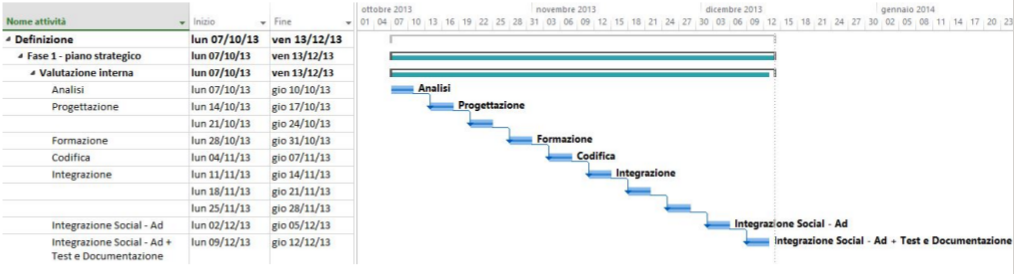
\includegraphics[scale=0.37]{/workspace/1911_up/Dropbox/thesis/Figures/tempo.png}
\caption[Pianificazione temporale]{Pianificazione temporale definita}
\label{pic-a}
\end{figure}

Il modello di ciclo di vita prescelto può essere paragonabile allo scrum: viene infatti preferito rispetto alla rigidità dei modelli più classici, in
quanto permetteva lo sviluppo continuo dei vari incrementi e la possibilità di mostrare
passo per passo i risultati ottenuti. Per chiarezza si riporta una breve descrizione degli
obiettivi presenti nel piano di lavoro che verranno maggiormente approfonditi nelle
sezioni successive:

\textbf{Obiettivo 1}: Studiare la fattibilità prestazionale di un software di rivelamento facciale e delle sue parti su un dispositivo mobile.

\textbf{Obiettivo 2}: Creazione di una libreria di appoggio ad OpenCV che renda di facile utilizzo il rilevamento facciale e delle parti presenti.

\textbf{Obiettivo 3}: Creazione di una libreria che permetta una facile condivisione dei contenuti multimediali eventualmente creati verso il social network Facebook.


%----------------------------------------------------------------------------------------

\section{Analisi}

In seguito allo studio del dominio applicativo effettuato durante le prime settimane di stage e alle spiegazioni del tutor aziendale sono stati individuati i requisiti del prototipo richiesto.
Dal momento che si tratta di un prototipo che dovrà essere alla base di una famiglia di prodotti, esso non sarà indipendente dall input umano ma dovrà garantire la flessibilità ed espandibilità necessaria.

Di seguito vengono riportati i casi d'uso principali individuati.

\subsection{Casi d'uso}

In questa sezione verranno elencati i casi d'uso del sistema che `e oggetto dello stage.
Dato che l'applicazione è stata pensata per rispondere solo alle azioni di un utente l'unico attore che prenderemo in
considerazione è l'utente utilizzatore. Per ogni caso d'uso verranno riportate:

\begin{itemize}
\item  \textit{Descrizione}: contenuto del caso d'uso
\item  \textit{Flusso principale degli eventi}
\item  \textit{Precondizioni}: asserzioni che sono valide prima dell'effettiva esecuzione del
caso d'uso
\item  \textit{Postcondizione}: asserzioni che sono valide dopo l'esecuzione del caso d'uso
\item  \textit{Postcondizione alternativa}: eventuali scenari alternativi che differiscono dal normale flusso del caso d'uso
\end{itemize}
Ogni caso d'uso ha un identificativo stile UCx dove x indica una posizione gerarchica.
Ogni caso d'uso è posizionato all'interno della gerarchia che parte dal caso d'uso più generale UC1 (radice dell'albero). Per ogni caso d'uso figlio valgono ovviamente le precondizioni del padre. Per chiarezza si definiscono gli acronimi per i termini RealTime (RT) e Static (S) per definire la duplice funzione dell'applicazione.

\subsubsection{UC1: Principale (RT)}

\textbf{\textit{Descrizione:}} L'utente ha avviato il programma, che risulta quindi pronto a rispondere agli eventuali input utente. L'utente può decidere lo Sprite da utilizzare.

\textbf{\textit{Flusso principale degli eventi:}} 

\begin{itemize}
\item L'utente può avviare il rilevamento del volto di parti facciali predefinite (UC1.1)
\item L'utente può calibrare la Camera (UC1.2)
\item L'utente può attivare la funzione di rilevamento di orientamento del volto (UC1.3)
\item L'utente può scegliere lo Sprite da utilizzare da una lista a schermo (UC1.4)
\end{itemize}

\textbf{\textit{Precondizione:}} L'applicazione è avviata e funzionante.


\begin{figure}[H]\centering  
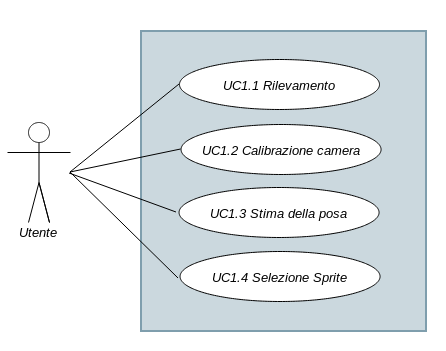
\includegraphics[scale=0.6]{/workspace/1911_up/Dropbox/thesis/Figures/uc1.png}
\caption[UC1 - Sistema]{UC1 - Sistema}
\label{pic-a}
\end{figure}


\subsubsection{UC2: Principale (S)}

\textbf{\textit{Descrizione:}} L'utente ha avviato il programma, che risulta quindi pronto a rispondere agli eventuali input utente. L'utente può decidere lo Sprite da utilizzare.

\textbf{\textit{Flusso principale degli eventi:}} 

\begin{itemize}
\item L'utente carica una foto dal dispositivo verso l'applicazione (UC2.1)
\item L'utente richiede la funzione di rilevamento del volto (UC2.2)
\item L'utente può scegliere lo Sprite da utilizzare da una lista a schermo (condiviso con UC2.3)
\end{itemize}

\textbf{\textit{Precondizione:}} L'applicazione è avviata e funzionante.

\begin{figure}[H]\centering  
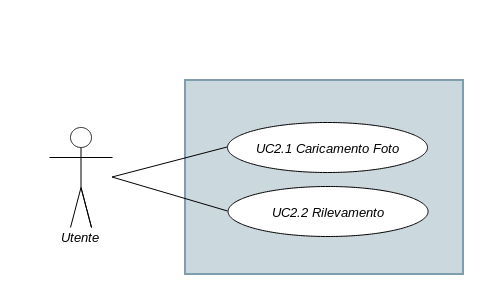
\includegraphics[scale=0.6]{/workspace/1911_up/Dropbox/thesis/Figures/uc2.png}
\caption[UC2 - Sistema]{UC2 - Sistema}
\label{pic-a}
\end{figure}


\subsubsection{UC3: Secondario}

\textbf{\textit{Descrizione:}} L'utente ha avviato il programma, ha scattato una foto in modalità dinamica o statica.

\textbf{\textit{Flusso principale degli eventi:}} 

\begin{itemize}
\item L'utente può ridimensionare la foto ottenuta in base a formati predefiniti (UC3.1)
\item L'utente può condividere la foto ottenuta verso applicazioni di messaggistica interne grazie al lancio di un Intent (UC3.2)
\item L'utente può effettuare il Login sulla piattaforma Facebook e condividere la foto su quest ultimo (UC3.3)
\end{itemize}

\textbf{\textit{Precondizione:}} L'applicazione è avviata e funzionante.

\begin{figure}[H]\centering  
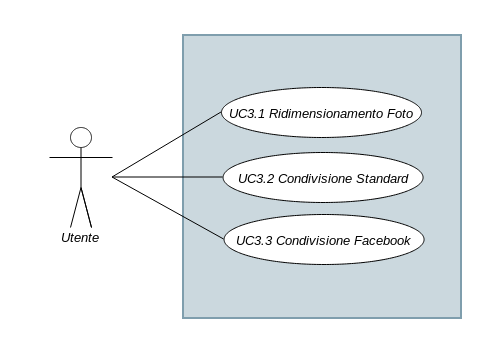
\includegraphics[scale=0.6]{/workspace/1911_up/Dropbox/thesis/Figures/uc3.png}
\caption[UC3 - Sistema]{UC3 - Sistema}
\label{pic-a}
\end{figure}


\subsubsection{UC1.1: (RT)::Rilevamento}

\textbf{\textit{Descrizione:}} L'utente può avviare il rilevamento del volto di parti facciali predefinite. L'applicazione reagisce con la creazione di templates che verranno successivamente riutilizzati per il tentativo di match sui frames successivi.


\textbf{\textit{Precondizione:}} L'applicazione è avviata e funzionante.
\textbf{\textit{Postcondizione:}} L'applicazione rileva gli eventuali volti presenti e le feature indicate.



\subsubsection{UC1.2: (RT)::Calibrazione Camera}

\textbf{\textit{Descrizione:}} 

\textbf{\textit{Flusso principale degli eventi:}} 

\begin{itemize}
\item L'utente può selezionare una camera (UC1.2.1)
\item L'utente può selezionare il tipo di elaborazione della camera (UC1.2.2)
\item L'utente può modificare la risoluzione del frame in ingresso (UC1.2.3)
\item L'utente può modificare la profondità di campionamento (distanza minima e massima su cui effettuare lo scan) (UC1.2.4)
\item L'utente può modificare il numero minimo di campionamenti sotto il quale il volto non viene riconosciuto come valido (UC1.2.5)
\item L'utente può abilitare/disabilitare lo scan delle parti facciali in tempo reale (UC1.2.6)
\item L'utente può abilitare/disabilitare la modalità alto contrasto e/o monocromatica (UC1.2.7)
\end{itemize}

\textbf{\textit{Precondizione:}} L'applicazione è avviata e funzionante. Inoltre l'utente ha espresso la volontà di utilizzare tale funzione attraverso la pressione di un bottone presente all'interno dell'interfaccia grafica.

\begin{figure}[H]\centering  
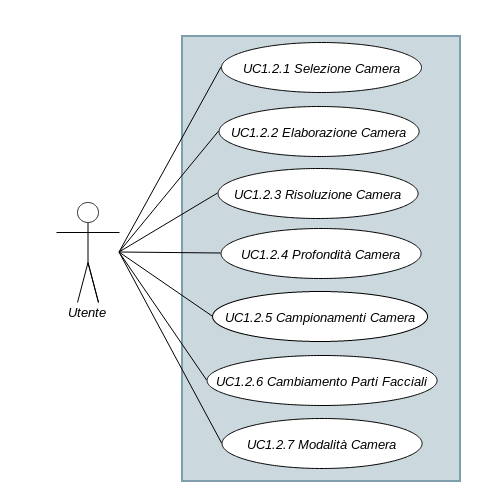
\includegraphics[scale=0.6]{/workspace/1911_up/Dropbox/thesis/Figures/uc12.png}
\caption[UC1.2 - Calibrazione camera]{UC1.2 - Calibrazione camera}
\end{figure}

\subsubsection{UC1.3: (RT)::Orientamento Volto}

\textbf{\textit{Descrizione:}} L'utente deve poter avviare la funzionalità che permette la triangolazione delle parti occhi-bocca per capire l'orientamento del volto in base alle fattezze dei triangolo individuato

\textbf{\textit{Postcondizione:}} L'applicazione rileverà in tempo reale l'orientamento del volto della persona rispetto alla camera grazie alla triangolazione delle parti occhi-bocca.


\subsubsection{UC1.4: (RT)::Selezione Sprite}

\textbf{\textit{Descrizione:}} L'utente può decidere quale tra i possibili Sprites utilizzare, da sovrapporre al volto individuato.

\textbf{\textit{Flusso principale degli eventi:}} 

\begin{itemize}
\item Caricamento all'interno di una ListView della lista di oggetti di tipo Sprite (UC1.4.1)
\item Selezione dello Sprite desiderato (UC1.4.2)
\item Effettiva renderizzazione dello Sprite che sarà posto in overlay su ogni fotogramma (UC1.4.3)
\end{itemize}

\textbf{\textit{Precondizione:}} L'applicazione è avviata e funzionante. Inoltre l'utente ha espresso la volontà di utilizzare tale funzione attraverso la pressione di un bottone presente all'interno dell'interfaccia grafica.

\begin{figure}[H]\centering  
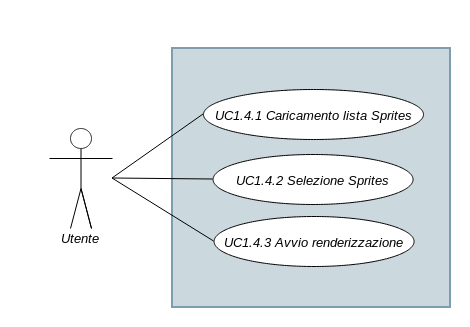
\includegraphics[scale=0.6]{/workspace/1911_up/Dropbox/thesis/Figures/uc14.png}
\caption[UC1.4 - Selezione Sprite]{UC3.3 - Selezione Sprite}
\label{pic-a}
\end{figure}

\subsubsection{UC2.1: (S)::Caricamento Foto}

\textbf{\textit{Descrizione:}} L'utente sceglie attraverso l'utilizzo di una galleria proprietaria di Android la foto da caricare.

\textbf{\textit{Postcondizione:}} L'applicazione carica al suo interno una foto proveniente dallo storage dello smartphone e la tiene in memoria.


\subsubsection{UC2.2: (S)::Rilevamento}

\textbf{\textit{Descrizione:}} L'utente può avviare il rilevamento del volto di parti facciali predefinite. L'applicazione reagisce con la creazione di un template del volto rilevato.


\textbf{\textit{Precondizione:}} L'applicazione è avviata e funzionante.
\textbf{\textit{Postcondizione:}} L'applicazione rileva gli eventuali volti presenti e le feature indicate.

\subsubsection{UC2.3: (S)::Selezione Sprite}

\textbf{\textit{Descrizione:}} L'utente può decidere quale tra i possibili Sprites utilizzare, da sovrapporre al volto individuato.

\textbf{\textit{Flusso principale degli eventi:}} 

\begin{itemize}
\item Caricamento all'interno di una ListView della lista di oggetti di tipo Sprite (UC1.4.1)
\item Selezione dello Sprite desiderato (UC1.4.2)
\item Effettiva renderizzazione dello Sprite che sarà posto in overlay su ogni fotogramma (UC1.4.3)
\end{itemize}

\textbf{\textit{Precondizione:}} L'applicazione è avviata e funzionante.

\subsubsection{UC3.1: Secondario::Ridimensionamento frame}

\textbf{\textit{Descrizione:}} L'utente può ridimensionare la foto ottenuta scegliendo tra formati predefiniti.

\textbf{\textit{Postcondizione:}} L'applicazione ridimensiona l'immagine in base alla dimensione definita dall'utente.


\subsubsection{UC3.2: Secondario::Condivisione Interna}

\textbf{\textit{Descrizione:}} L'utente può condividere la foto ottenuta verso applicazioni di messaggistica

\textbf{\textit{Flusso principale degli eventi:}} 

\begin{itemize}
\item L'utente deve poter esprimere il suo intento cliccando su un tasto presente all'interno dell'interfaccia grafica (UC3.2.1)
\item L'applicazione deve esporre i mezzi attraverso i quali il contenuto multimediale può essere condiviso (UC3.2.2)
\item L'applicazione condivide il contenuto multimediale in seguito alla selezione dell'utente (UC3.2.3)
\end{itemize}

\textbf{\textit{Precondizione:}} L'applicazione è avviata e funzionante.


\begin{figure}[H]\centering  
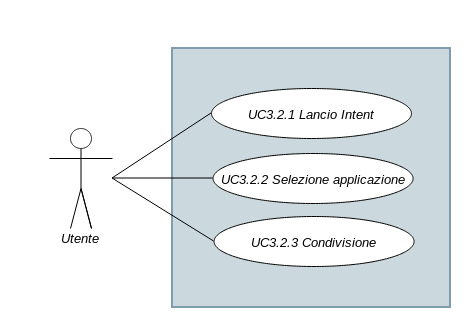
\includegraphics[scale=0.6]{/workspace/1911_up/Dropbox/thesis/Figures/uc32.png}
\caption[UC3.2 - Condivisione Interna]{UC3.2 - Condivisione Interna}
\label{pic-a}
\end{figure}

\subsubsection{UC3.3: Secondario::Facebook}

\textbf{\textit{Descrizione:}} L'utente ha avviato il programma, ha scattato una foto in modalità dinamica o statica.

\textbf{\textit{Flusso principale degli eventi:}} 

\begin{itemize}
\item L'utente può effettuare il login su facebook. (UC3.3.1)
\item L'utente può inserire un messaggio da allegare alla foto. (UC3.3.2)
\item L'utente può condividere tale contenuto sulla propria "bacheca" o su quella di altri conoscenti. (UC3.3.3)
\end{itemize}

\textbf{\textit{Postcondizione alternativa:}} L'applicazione è avviata e funzionante.


\begin{figure}[H]\centering  
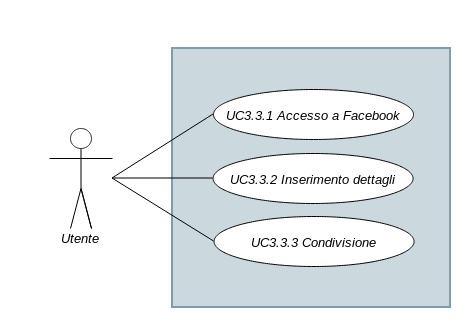
\includegraphics[scale=0.6]{/workspace/1911_up/Dropbox/thesis/Figures/uc33.png}
\caption[UC3.3 - Condivisione Facebook]{UC3.3 - Condivisione Facebook}
\label{pic-a}
\end{figure}

\subsubsection{UC1.2.1: (RT)::Calibrazione Camera::Selezione Camera}

\textbf{\textit{Descrizione:}} L'utente ha la possibilità di selezionare tra le camere presenti all'interno del dispositivo,se disponibili. 

\textbf{\textit{Postcondizione:}} L'applicazione ha accesso all'utilizzo della camera.

\textbf{\textit{Postcondizione alternativa:}} L'applicazione non ha accesso all'utilizzo della camera.

\subsubsection{UC1.2.2: (RT)::Calibrazione Camera::Elaborazione Camera}

\textbf{\textit{Descrizione:}} L'utente ha la possibilità di selezionare che tipo di camera utilizzare (Nativa OpenCV o Android) 

\textbf{\textit{Postcondizione:}} L'applicazione utilizzerà da quel momento il tipo di camera input selezionato

\subsubsection{UC1.2.3: (RT)::Calibrazione Camera::Risoluzione Camera}

\textbf{\textit{Descrizione:}} L'utente ha la possibilità di selezionare la risoluzione alla quale scalare il frame in ingresso.

\textbf{\textit{Postcondizione:}} L'applicazione scalerà ogni frame in ingresso alla risoluzione indicata dall'utente, mantenendo l'aspect ratio.

\subsubsection{UC1.2.4: (RT)::Calibrazione Camera::Profondità Camera}

\textbf{\textit{Descrizione:}}  L'utente ha la possibilità di selezionare la dimensione minima e massima (range operativo) secondo le quali il campionamento va effettuato.

\textbf{\textit{Postcondizione:}} L'applicazione effettuerà il campionamento nel range definito.

\subsubsection{UC1.2.5: (RT)::Calibrazione Camera::Campionamenti Camera}

\textbf{\textit{Descrizione:}} L'utente ha la possibilità di selezionare il numero di campionamenti al di sotto del quale il volto rilevato viene valutato come non valido e quindi scartato.

\textbf{\textit{Postcondizione:}} L'applicazione effettua lo scan del frame basandosi sul numero di campionamenti settato dall'utente, al di sotto del quale il volto rilevato viene valutato come non valido e quindi scartato. 

\subsubsection{UC1.2.6: (RT)::Calibrazione Camera::Parti Facciali}

\textbf{\textit{Descrizione:}} L'utente ha la possibilità di selezionare quali parti facciali abilitare.

\textbf{\textit{Postcondizione:}} L'applicazione eseguirà la ricerca di tutte le parti impostate dall'utente.

\subsubsection{UC1.2.7: (RT)::Calibrazione Camera::Modalità Camera}

\textbf{\textit{Descrizione:}} L'utente ha la possibilità di decidere se il frame in ingresso deve essere riconvertito in un immagine monocromatica e/o se esso debba subire un'elaborazione atta ad elevarne il contrasto.

\textbf{\textit{Postcondizione:}} L'applicazione applicherà la modalità definita.

\subsubsection{UC1.4.1: (RT)::Selezione Sprite::Caricamento Sprites}

\textbf{\textit{Descrizione:}} L'applicazione deve permettere su richiesta il caricamento su una ListView della lista di oggetti di tipo Sprite.

\textbf{\textit{Postcondizione:}} L'applicazione popola, attraverso l'utilizzo di un adapter, la ListView presente all'interno dell'interfaccia grafica.

\subsubsection{UC1.4.2: (RT)::Selezione Sprite::Selezione Sprites}

\textbf{\textit{Descrizione:}} L'applicazione deve permettere la selezione dello Sprite desiderato.

\textbf{\textit{Postcondizione:}} L'applicazione terrà in memoria lo Sprite selezionato, pronto per l'effettivo render.

\subsubsection{UC1.4.3: (RT)::Selezione Sprite::Visione Sprites}

\textbf{\textit{Descrizione:}} L'applicazione deve permettere l'effettiva renderizzazione dello Sprite che sarà posto in overlay su ogni fotogramma.

\textbf{\textit{Postcondizione:}} L'applicazione renderizza lo sprite in overlay, su ogni fotogramma, in corrispondenza del volto rilevato.

\subsubsection{UC3.2.1: Secondario::Condivisione Interna::Intent }

\textbf{\textit{Descrizione:}} L'utente deve poter esprimere il suo intento cliccando su un tasto presente all'interno dell'interfaccia grafica.

\textbf{\textit{Postcondizione:}} L'applicazione prepara l'adapter per il caricamento delle applicazioni di condivisione e popola la ListView.

\subsubsection{UC3.2.2: Secondario::Condivisione Interna::Selezione}

\textbf{\textit{Descrizione:}} L'applicazione deve esporre i mezzi attraverso i quali il contenuto multimediale può essere condiviso.

\textbf{\textit{Postcondizione:}} L'applicazione rende visibile a schermo gli le applicazioni disponibili.

\subsubsection{UC3.2.3: Secondario::Condivisione Interna::Condivisione}

\textbf{\textit{Descrizione:}} L'applicazione deve rispondere alla scelta dell'utente di utilizzare quella particolare applicazione per la condivisione del contenuto multimediale.

\textbf{\textit{Postcondizione:}} L'applicazione condivide il contenuto multimediale in seguito alla selezione dell'utente.

\subsubsection{UC3.3.1: Secondario::Facebook::Login}

\textbf{\textit{Descrizione:}} L'utente può inoltrare la richiesta di accesso alla piattaforma Facebook attraverso l'uso di un bottone presente all'interno dell'interfaccia grafica.

\textbf{\textit{Postcondizione:}} L'utente ha accesso alla piattaforma con i dovuti permessi. La classe si impegna di mantenere in memoria la sessione attiva 

\textbf{\textit{Postcondizione alternativa:}} L'utente non ha accesso alla piattaforma e viene invitato a controllare i dati di accesso.

\subsubsection{UC3.3.2: Secondario::Facebook::Messaggio}

\textbf{\textit{Descrizione:}} L'utente può scegliere se aggiungere un messaggio testuale alla foto .

\textbf{\textit{Postcondizione:}} L'utente ha inserito un messaggio testuale che sarà preso in consegna al momento dell'eventuale invio dei contenuti.

\textbf{\textit{Postcondizione alternativa:}} L'utente non ha inserito un messaggio testuale.

\subsubsection{UC3.3.3: Secondario::Facebook::Condivisione}

\textbf{\textit{Descrizione:}} L'utente può scegliere se la destinazione della foto sarà la propria "bacheca" o quella di altri conoscenti.

\textbf{\textit{Postcondizione:}} L'utente carica con successo il contenuto.

\textbf{\textit{Postcondizione alternativa:}} Il contenuto non viene caricato per problemi di connessione verso la piattaforma.



\subsection{Associazione Requisiti-Casi d'uso}

La classificazione dei requisiti sarà seguirà il formalismo:
\begin{center}
	\textbf{R\{TIPO\}\{RICHIESTA\}\{GERARCHIA\}}
\end{center}

Nello specifico:
\begin{itemize}
\item TIPO può essere:
	\begin{itemize}
		\item F, indica un requisito funzionale
		\item Q, indica un requisito di qualità
		\item V, indica un requisito di vincolo
	\end{itemize} 
\item IMPEGNO può essere:
	\begin{itemize}
		\item O, indica un requisito obbligatorio
		\item D, indica un requisito desiderabile
	\end{itemize} 
\item GERARCHIA: i requisiti sono organizzati gerarchicamente secondo una struttura ad albero. Se la complessità di un requisito viene ritenuta elevata, questo può essere diviso in sotto-requisiti.
\end{itemize}

A seguire i requisiti individuati:

\begin{center}
    \begin{longtable}{ | p{2cm} | p{7cm} | p{2cm} |}
    \hline
    Requisiti & Descrizione & Caso d'uso \\ \hline
    RFO1 &  L'applicazione deve permettere il rilevamento facciale in tempo reale su dispositivi mobili Android & UC1  \\ \hline 
    RFO1.1 &  L'utente può avviare il rilevamento del volto di parti facciali predefinite. L'applicazione reagisce con la creazione di templates che verranno successivamente riutilizzati per il tentativo di match sui frames successivi  & UC1.1 \\ \hline
    RFO1.2 &  L'applicazione deve permettere di calibrare la camera corrente  & UC1.2  \\ \hline 
    RFO1.2.1 &  L'applicazione deve permettere all'utente di selezionare la camera desiderata & UC1.2.1  \\ \hline
    RFO1.2.2 &  L'applicazione deve permettere all'utente di modificare il tipo di elaborazione della camera & UC1.2.2  \\ \hline
    RFO1.2.3 &  L'applicazione deve permettere all'utente di modificare la risoluzione del frame in ingresso & UC1.2.3  \\ \hline
    RFO1.2.4 &  L'applicazione deve permettere all'utente di modificare la profondità di campionamento (distanza minima e massima su cui effettuare lo scan) & UC1.2.4  \\ \hline
    RFO1.2.5 &  L'applicazione deve permettere all'utente di modificare il numero minimo di campionamenti sotto il quale il volto non viene riconosciuto come valido  & UC1.2.5  \\ \hline
    RFO1.2.6 &  L'applicazione deve permettere all'utente di abilitare di abilitare/disabilitare la ricerca delle parti in tempo reale  & UC1.2.6  \\ \hline
    RFO1.2.7 &  L'applicazione deve permettere all'utente di abilitare/disabilitare la modalità contrasto e/o monocromatica  & UC1.2.7  \\ \hline
    RFD1.3 &  L'applicazione deve permettere di cogliere l'orientamento dell'eventuale volto individuato & UC1.3 \\ \hline    
    RFD1.4 &  L'applicazione deve permettere di scegliere lo Sprite da utilizzare & UC1.4 \\ \hline
    RFO1.4.1 &  L'applicazione deve caricare una lista di Sprites, che saranno successivamente selezionabili dall'utente & UC1.4.1  \\ \hline
    RFO1.4.2 &  L'applicazione deve permettere all'utente di selezionare uno o più Sprites desiderati da una ListView presente all'interno dell'interfaccia grafica  & UC1.4.2  \\ \hline
    RFO1.4.3 &  L'applicazione deve poter renderizzare gli Sprites precedentemente selezionati & UC1.4.3  \\ \hline    
    RFO2 &  L'applicazione deve permettere di rilevare volti a partire da un immagine statica su dispositivi mobili Android & UC2  \\ \hline
    RFO2.1 &  L'applicazione deve permettere all'utente di caricare una foto dal proprio smartphone & UC2.1  \\ \hline 
    RFO2.2 &  L'applicazione deve permettere di avviare il rilevamento facciale & UC2.2 \\ \hline
    RFD2.3 &   L'applicazione deve permettere di scegliere uno o più Sprites da utilizzare  & UC2.3  \\ \hline 
    RFO3 &  L'applicazione deve permettere la condivisione di contenuti multimediali & UC3 \\ \hline
    RFD3.1 &  L'applicazione deve permettere di ridimensionare la foto scattata in base a formati predefiniti & UC3.1 \\ \hline
    RFD3.2 &  L'applicazione deve permettere di condividere la foto ottenuta verso applicazioni di messaggistica interne  & UC3.2 \\ \hline
    RFD3.2.1 &  L'applicazione deve fornire l'utente di un bottone attraverso il quale può esprimere il suo intento di condividere il contenuto  & UC3.2.1 \\ \hline
    RFD3.2.2 &  L'applicazione deve rispondere fornendo graficamente una risposta contenente i servizi di inoltro disponibili  & UC3.2.2 \\ \hline
    RFD3.2.3 &  L'applicazione deve condividere il contenuto multimediale attraverso il servizio selezionato  & UC3.2.3 \\ \hline    
    RFD3.3 &  L'applicazione deve permettere il login facebook e condividere la foto su quest ultimo  & UC3.3 \\ \hline
    RFD3.3.1 &  L'applicazione deve permettere l'inoltro di una richiesta di accesso verso i server Facebook ed il mantenimento della sessione attiva & UC3.3.1 \\ \hline
    RFD3.3.2 &  L'applicazione deve permettere l'inserimento di un testo da allegare alla foto & UC3.3.2 \\ \hline
    RFD3.3.3 &  L'applicazione deve permettere il caricamento della foto sulla piattaforma Facebook & UC3.3.3 \\ \hline
    RFD4 &  L'applicazione deve mantenere un framerate minimo di 15 fotogrammi al secondo & non mappabile \\ \hline
    \end{longtable}
    \end{center}
    \textbf{Appunto RFD4}: Un sistema è scalabile se può essere adattato a diversi contesti con forti differenze di complessità senza che questo richieda la riprogettazione dello stesso sistema. Si richiede che le prestazioni di un sistema possano essere aumentate "semplicemente" fornendo al sistema stesso maggiori risorse di calcolo. Nello specifico si richiede che il sistema mantenga il framerate minimo indicato per gli smartphone Android aventi sistema operativo uguale o successivo ad \textit{HoneyComb}.


